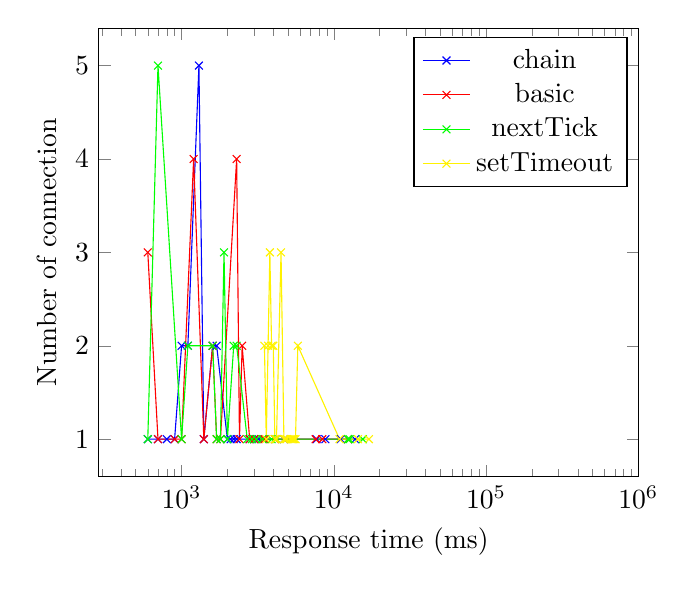
\begin{tikzpicture}
\begin{semilogxaxis}[xmin=0,xmax=1000000, ylabel=Number of connection, xlabel=Response time (ms)]
\addplot[color=blue, mark=x] coordinates {(600,1)(700,1)(800,1)(900,1)(1000,2)(1100,2)(1300,5)(1400,1)(1600,2)(1700,2)(2000,1)(2100,1)(2200,1)(2300,1)(2800,1)(3000,1)(3200,1)(4700,1)(7700,1)(8800,1)(11100,1)(13800,1)};
\addplot[color=red, mark=x] coordinates {(600,3)(700,1)(900,1)(1000,1)(1200,4)(1400,1)(1600,2)(1700,1)(1800,1)(2300,4)(2400,1)(2500,2)(2800,1)(3000,1)(3400,1)(3500,1)(4100,1)(7600,1)(8400,1)(12400,1)};
\addplot[color=green, mark=x] coordinates {(600,1)(700,5)(1000,1)(1100,2)(1600,2)(1700,1)(1800,1)(1900,3)(2000,1)(2200,2)(2300,2)(2700,1)(2900,1)(3100,1)(3400,1)(3900,1)(4200,1)(12400,1)(12700,1)(15500,1)};
\addplot[color=yellow, mark=x] coordinates {(3500,2)(3600,1)(3700,2)(3800,3)(3900,2)(4000,2)(4100,1)(4200,1)(4500,3)(4700,1)(4800,1)(4900,1)(5200,1)(5300,1)(5400,1)(5500,1)(5600,1)(5800,2)(10900,1)(14400,1)(17000,1)};
\legend{chain, basic, nextTick, setTimeout}
\end{semilogxaxis}
\end{tikzpicture}
